%%%%%%%%%%%%%%%%%%%%%%%%%%%%%%%%%%%%%%%%%
% Social Media Mining Poster (CE7066)
% Extending InfoOpsGFM (AAAI 2025)
% ---------------------------------------
% Template based on NIWeek 2014 Poster by T. Reveyrand
% Original template created by Brian Amberg (baposter@brian-amberg.de)
%%%%%%%%%%%%%%%%%%%%%%%%%%%%%%%%%%%%%%%%%

% A1 size. fontscale=0.44 (= 0.292 * 841/594) keeps the base layout
% identical to the original A0 design, scaled down proportionally to A1.
\documentclass[a1paper,portrait,fontscale=0.44]{baposter}

\usepackage[font=small,labelfont=bf]{caption} % Required for specifying captions to tables and figures
\usepackage{booktabs} % Horizontal rules in tables
\usepackage{relsize} % Used for making text smaller in some places
\usepackage{amsmath,amsfonts,amssymb,amsthm} % Math packages
\usepackage{eqparbox}
\usepackage{textcomp}
\usepackage{graphicx}

\graphicspath{{figures/}} % Directory in which figures are stored

% Premium Harmonized Color Palette
\definecolor{bordercol}{RGB}{44,62,80}      % Dark Slate Blue
\definecolor{headercol1}{RGB}{26,188,156}   % Emerald Teal (Left side of header)
\definecolor{headercol2}{RGB}{52,73,94}     % Dark Slate Gray (Right side of header)
\definecolor{headerfontcol}{RGB}{255,255,255} % White header text
\definecolor{boxcolor}{RGB}{248,249,249}    % Very light gray content boxes

\begin{document}

\background{ % Set the background to a clean layout
\begin{tikzpicture}[remember picture,overlay]
\draw (current page.north west)+(-2em,2em) node[anchor=north west]
{
\includegraphics[height=1.1\textheight]{background}};
\end{tikzpicture}
}

\begin{poster}{
grid=false,
borderColor=bordercol,
headerColorOne=headercol1,
headerColorTwo=headercol2,
headerFontColor=headerfontcol,
boxColorOne=boxcolor,
headershape=roundedright,
headerfont=\Large\sf\bf,
textborder=rectangle,
background=user,
headerborder=open,
boxshade=plain
}

%
%----------------------------------------------------------------------------------------
%	TITLE AND AUTHOR NAME
%----------------------------------------------------------------------------------------
%
{ \bf  \huge {IOHunter+: Coverage-Gated Channel-Specific Alignment} \\
  \Large \it Improving Cross-Country Zero-Shot IO Account Detection under Sparse Behavioral Networks} % Poster title
{\vspace{0.3em} \smaller CE7066 Social Media Mining --- Final Project of Group 7 \\
  \smaller Hsieh-Yu Yang, Terry Tan, Chien-Ting Kuo, Dinh Minh Toan\\
\smaller\it Department of Computer Science \& Information Engineering\\
International Graduate Program in Artificial Intelligence\\
National Central University}
{
\includegraphics[scale=0.3]{NI.jpg}} % University/lab logo

%----------------------------------------------------------------------------------------
%	INTRODUCTION
%----------------------------------------------------------------------------------------
\headerbox{1. Introduction}{name=introduction,column=0,row=0, span=3}{
\begin{itemize}
\item \textbf{Task}: Cross-country zero-shot Information Operations (IO) account detection. The model is trained on a set of source countries (with labels) and directly transferred to a held-out target country.
\item \textbf{Input Modalities}: Text features (SBERT semantic embeddings from tweets) and graph structures (5 coordinate sub-networks: Retweet, URL sharing, Hashtag sequence, Fast retweet, and Tweet text similarity).
\item \textbf{Dataset}: Six country-level Twitter/X IO campaign graphs released with IOHunter (UAE, Cuba, Russia, Venezuela, Iran, China), each containing 666--22{,}694 accounts labeled as IO drivers vs.\ legitimate users.
\item \textbf{Extension of AAAI 2025 (IOHunter)}: IOHunter effectively integrates text and network information for cross-country IO detection, but its fused similarity network may combine high-coverage and low-coverage behavioral channels into a single graph. Our analysis indicates that this can weaken transferable coordination signals on sparse target graphs. To address this limitation, we propose \textbf{CS-DFA} with \textbf{Coverage-Gated Fusion}.
\end{itemize}
}

%----------------------------------------------------------------------------------------
%	THE LOW-COVERAGE NOISE DILUTION CHALLENGE (LEFT COLUMN, TOP)
%----------------------------------------------------------------------------------------
\headerbox{2. Evolution of Zero-Shot}{name=challenges,column=0,below=introduction}{
\small
\begin{itemize}
\item \textbf{InfoOpsGFM (AAAI'25 Baseline)}: Transferred a basic Multimodal GNN directly across countries. It suffered from massive domain gaps due to varying country profiles.
\item \textbf{DFA (Decoupled Feature Alignment)}: Aligned domains explicitly by decoupling text and structural representations via cross-attention.
\item \textbf{NHS + TAVS (Ours)}: Developed Neighborhood Smoothing (NHS) and Target-Adaptive Validation Thresholding (TAVS) to address local topology shifts and class prior imbalances in target countries.
\item \textbf{The Merging Bottleneck}: All prior models merge all five behavioral sub-networks into a single homogeneous graph. In target countries with low sub-network coverage (e.g., China has only 3--7\% coverage for hashtag sharing and fast retweets), 93\%+ of nodes become isolated in these channels. Running a single GNN over the merged graph forces these isolated nodes to propagate massive noise, severely diluting the coordination signal of primary channels (coRT/coURL).
\end{itemize}
}

%----------------------------------------------------------------------------------------
%	COVERAGE-GATED FUSION (LEFT COLUMN, MIDDLE)
%----------------------------------------------------------------------------------------
\headerbox{4. Coverage-Gated Fusion}{name=fusion,column=0,below=challenges}{
\small
To prevent isolated nodes from propagating noise, we define a binary coverage mask $M[n, c] \in \{0, 1\}$ recording if node $n$ participates in sub-network channel $c$.

\textbf{Mathematical Formulation}:
For node $n$ and channel embedding $Z_c(n)$:
\[
\scalebox{0.72}{$
\text{Score}(n, c) =
\begin{cases}
\text{Att}(Z_c(n)) + \lambda \log(\text{Cov}_c), & M[n, c] = 1 \\
-\infty, & M[n, c] = 0
\end{cases}$}
\]
where $\lambda$ controls the \textbf{Coverage Prior}. Normalization is done via softmax:
\[
\scalebox{0.75}{$
\alpha_n = \text{Softmax}(\text{Score}(n, \cdot))
\qquad
Z_{\text{fused}}(n) = \sum_{c} \alpha_{n, c} Z_c(n)$}
\]
This ensures nodes only aggregate and fuse features from behavioral networks they actively belong to.
}

%----------------------------------------------------------------------------------------
%	KEY FINDINGS (LEFT COLUMN, BOTTOM)
%----------------------------------------------------------------------------------------
\headerbox{6. Key Findings}{name=findings,column=0,below=fusion,above=bottom}{
\small
\begin{itemize}
\item \textbf{CS-DFA wins across all countries}: Outperforms Paper Baseline and DFA by a large margin (6-country Average F1-Macro: \textbf{0.775 $\rightarrow$ 0.952}, +17.7\%).
\item \textbf{Decisive Gating Contribution}: Disabling the coverage gate collapses performance to \textbf{0.686} (worse than DFA), verifying that channel-splitting is harmful without gated noise filtering.
\item \textbf{Inert Prior \& Alignment}: Ablation results show that domain alignment (CORAL) and additive coverage priors have negligible impacts compared to the critical gating mechanism.
\end{itemize}
}

%----------------------------------------------------------------------------------------
%	METHODOLOGY (RIGHT COLUMN, TOP)
%----------------------------------------------------------------------------------------
\headerbox{3. CS-DFA Model Architecture}{name=methodology,span=2,column=1,below=introduction}{
CS-DFA separates the five behavior networks into independent channels and applies coverage-gated attention.
\begin{center}
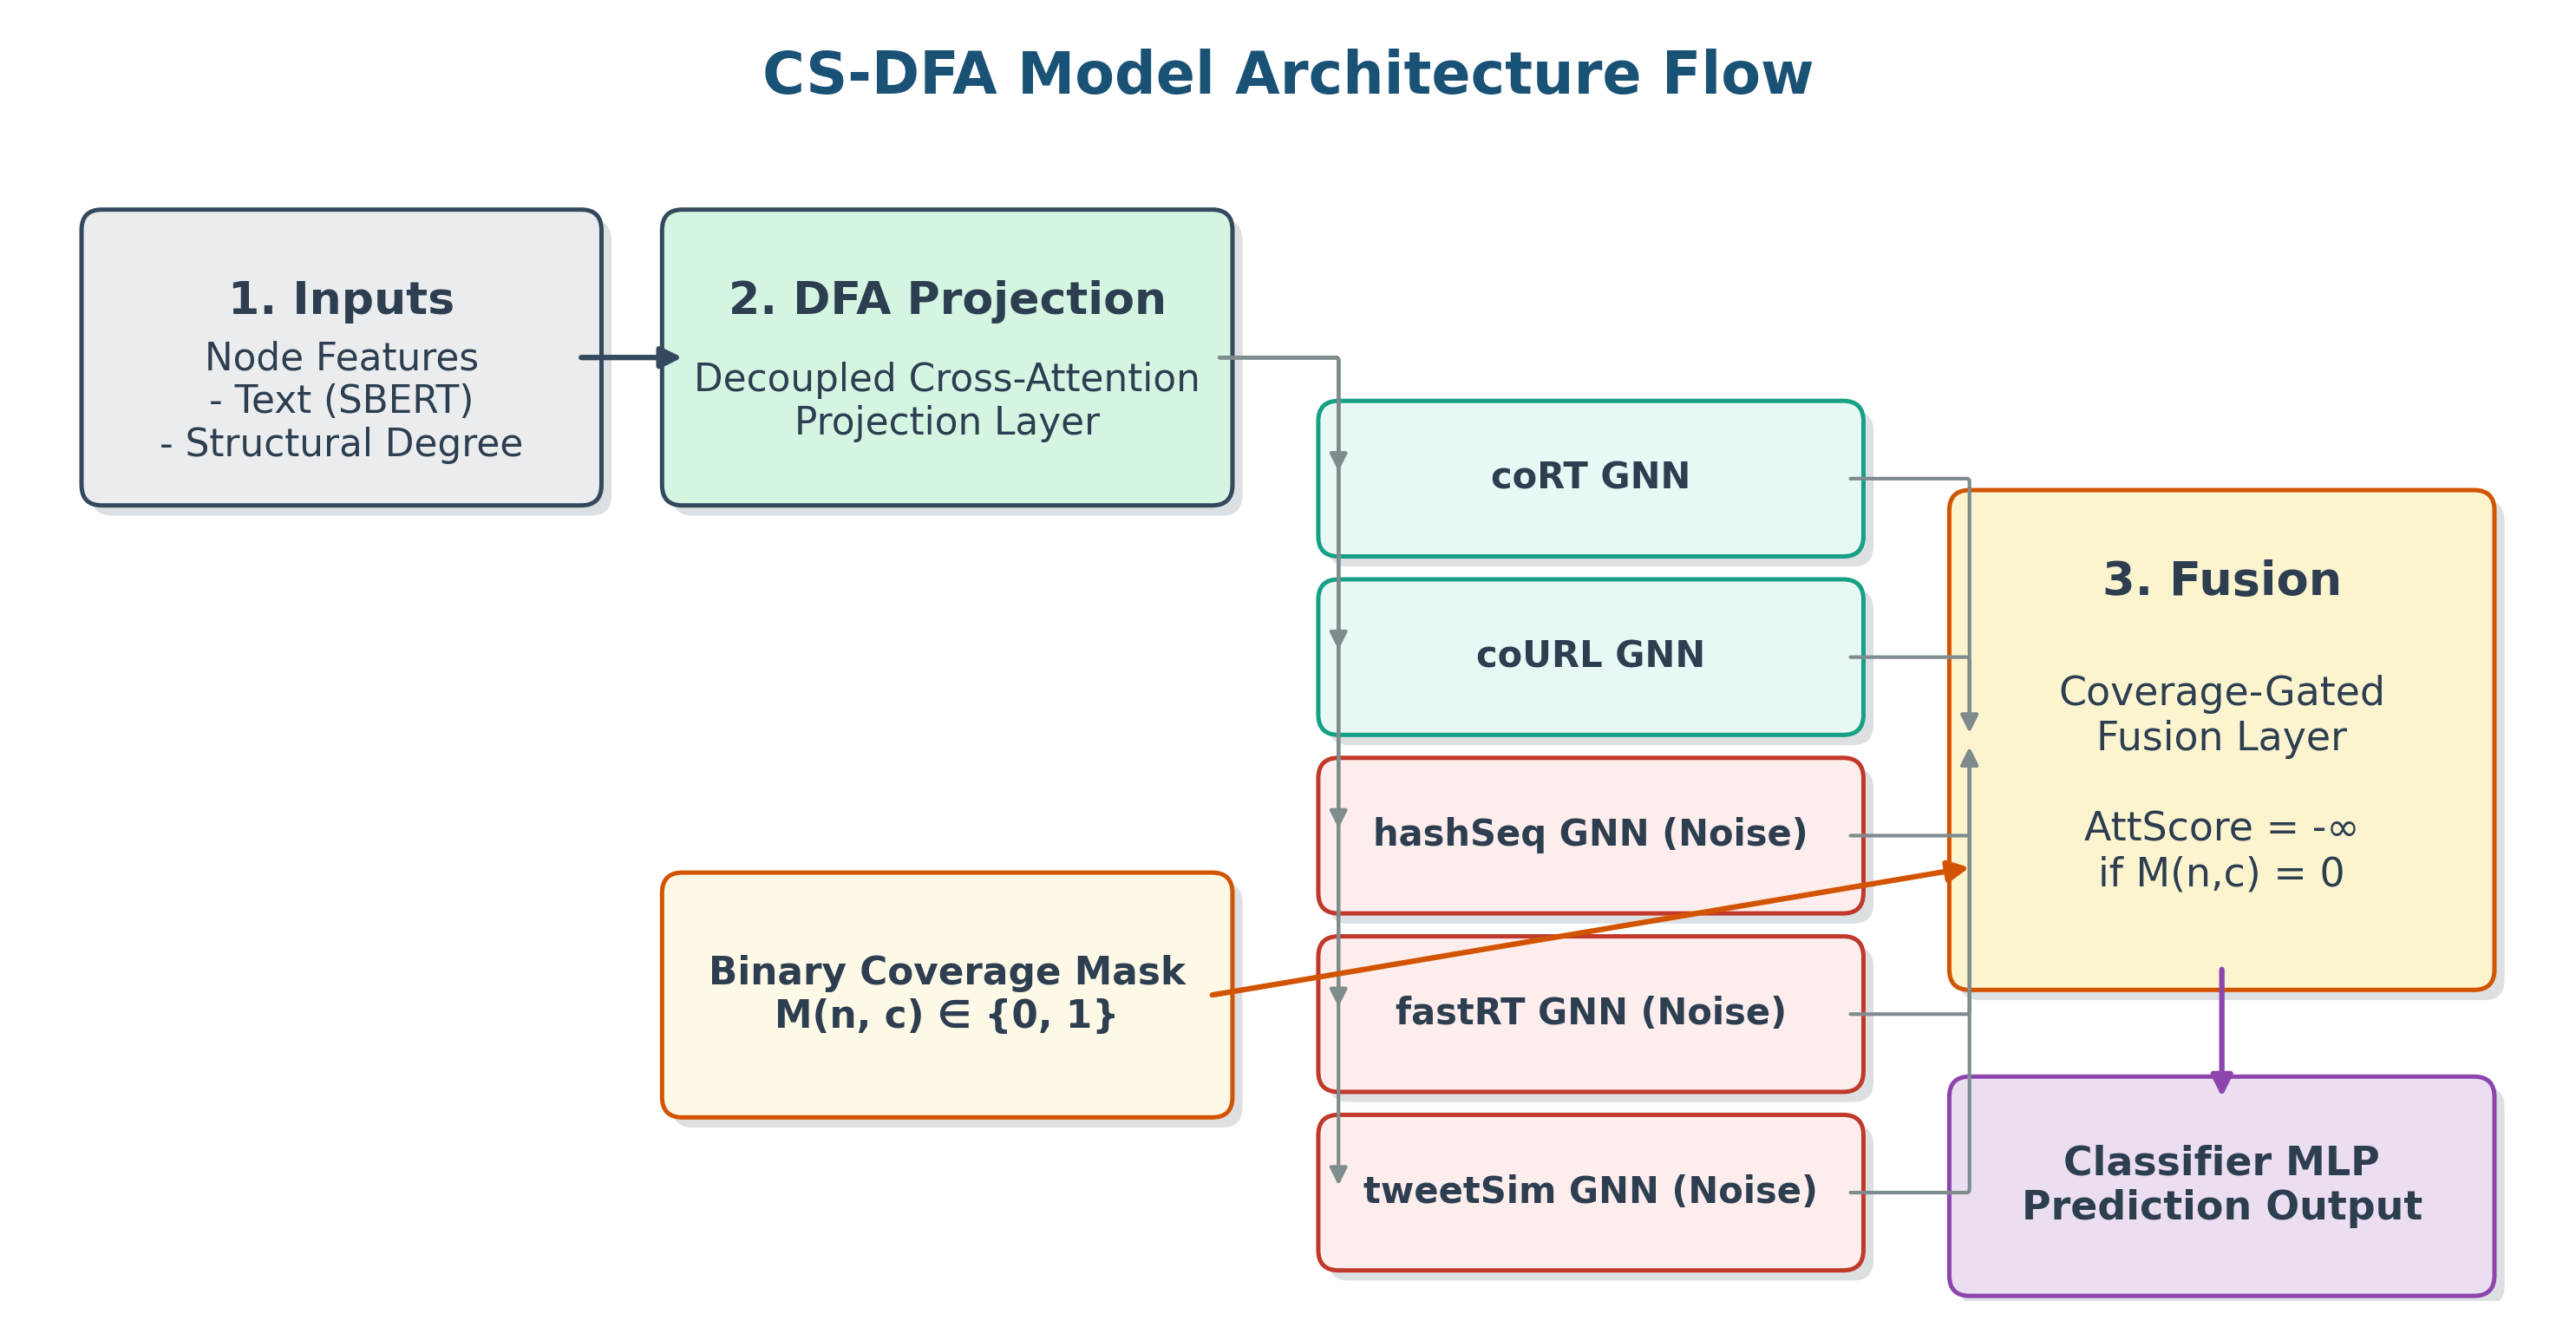
\includegraphics[width=0.92\linewidth]{poster_architecture_flow1}
\end{center}
\begin{enumerate}
\item \textbf{DFA Projection}: Multimodal node features are projected using a decoupled cross-attention module.
\item \textbf{Channel-Specific GNNs}: Instead of a single GNN on a merged graph, we run \textbf{five independent ChannelGNNs} (one for each sub-network: coRT, coURL, hashSeq, fastRT, tweetSim).
\item \textbf{Coverage-Gated Fusion}: Merges channel embeddings dynamically based on node active presence.
\end{enumerate}
}

%----------------------------------------------------------------------------------------
%	EXPERIMENTAL RESULTS (RIGHT COLUMN, BOTTOM)
%----------------------------------------------------------------------------------------
\headerbox{5. Experimental Results}{name=results,span=2,column=1,below=methodology,above=bottom}{
We evaluate zero-shot cross-country transfer on 6 target countries. CS-DFA consistently outperforms all
baselines.
\begin{center}
\vspace{-0.1cm}
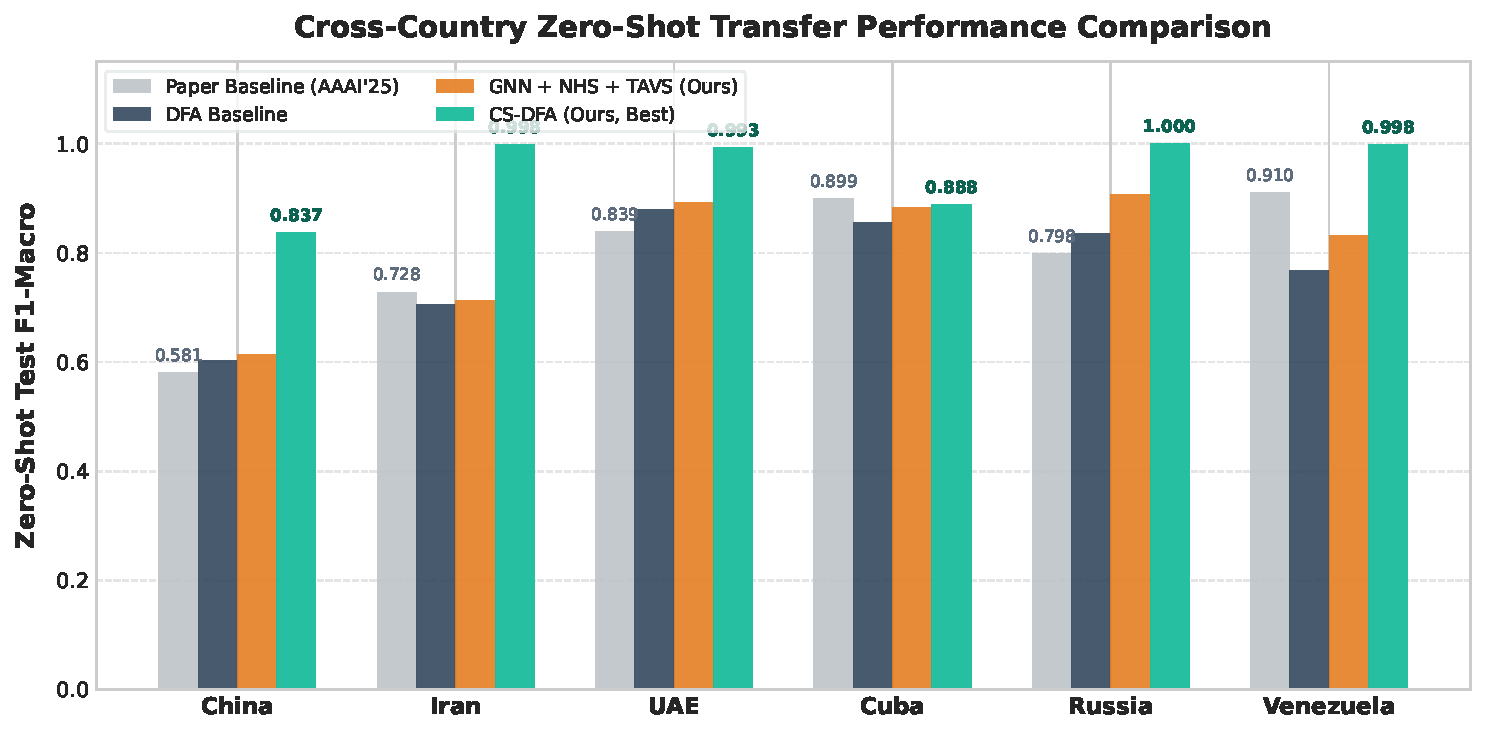
\includegraphics[width=0.80\linewidth]{poster_results_comparison}
\vspace{-0.25cm}
\end{center}

\textbf{Ablation Analysis} (Averaged 6-Country F1-Macro):
  \vspace{-0.15cm}
  {\centering
  \resizebox{0.86\linewidth}{!}{\begin{tabular}{l c c c c}
  \toprule
  \textbf{Variant} & \textbf{Gating} & \textbf{Prior $\lambda$} & \textbf{CORAL} & \textbf{Avg F1-Macro} \\
  \midrule
  \textbf{CS-DFA (Full)} & \textbf{ON} & 1.0 & Channel & \textbf{0.952} \\
  \textbf{No CORAL} & ON & 1.0 & OFF & 0.950 \\
  \textbf{No Prior} & ON & 0.0 & Channel & 0.952 \\
  \textbf{No Gating (nogate)} & \textbf{OFF} & 0.0 & OFF & \textbf{0.686} \\
  DFA Baseline & -- & -- & -- & 0.775 \\
  \bottomrule
  \end{tabular}}\par}
  \vspace{0.1cm}
}

\end{poster}

\end{document}